% mnras_template.tex 
%
% LaTeX template for creating an MNRAS paper
%
% v3.0 released 14 May 2015
% (version numbers match those of mnras.cls)
%
% Copyright (C) Royal Astronomical Society 2015
% Authors:
% Keith T. Smith (Royal Astronomical Society)

% Change log
%
% v3.0 May 2015
%    Renamed to match the new package name
%    Version number matches mnras.cls
%    A few minor tweaks to wording
% v1.0 September 2013
%    Beta testing only - never publicly released
%    First version: a simple (ish) template for creating an MNRAS paper

%%%%%%%%%%%%%%%%%%%%%%%%%%%%%%%%%%%%%%%%%%%%%%%%%%
% Basic setup. Most papers should leave these options alone.
\documentclass[fleqn,usenatbib]{mnras}

% MNRAS is set in Times font. If you don't have this installed (most LaTeX
% installations will be fine) or prefer the old Computer Modern fonts, comment
% out the following line
\usepackage{newtxtext,newtxmath}
% Depending on your LaTeX fonts installation, you might get better results with one of these:
%\usepackage{mathptmx}
%\usepackage{txfonts}

% Use vector fonts, so it zooms properly in on-screen viewing software
% Don't change these lines unless you know what you are doing
\usepackage[T1]{fontenc}
\usepackage{ae,aecompl}


\usepackage{graphicx}
\usepackage{amsmath}
\usepackage{amssymb}
\usepackage{amsfonts}
%\usepackage{wasysym}
\usepackage{natbib}
\usepackage{graphicx}
\usepackage{epsfig}
%\usepackage{epstopdf}
% bibliography and bibfile journal definitions (taken from aa.cls)

% Astronomy and Astrophysics
\def\aj{AJ}					% Astronomical Journal
\def\araa{ARA\&A}				% Annual Reviews of Astronomy and Astrophysics
\def\apj{ApJ}					% Astrophysical Journal
\def\apjl{ApJL}					% Astrophysical Journal, Letters
\def\apjs{ApJS}					% Astrophysical Journal, Supplement Series
\def\apss{Ap\&SS}				% Astrophysics & Space Science
\def\capsp{Comments on Astrophysics and Space Physics}
\def\aap{A\&A}					% Astronomy and Astrophysics
\def\aapr{A\&A~Rev.}				% Astronomy and Astrophysics Reviews
\def\aaps{A\&AS}				% Astronomy and Astrophysics, Supplement
\def\azh{AZh}					% Astronomicheskii Zhurnal
\def\baas{BAAS}					% Bulletin of the AAS
\def\jrasc{JRASC}				% Journal of the RAS of Canada
\def\memras{MmRAS}				% Memoirs of the RAS
\def\mnras{MNRAS}				% Monthly Notices of the Royal Astronomical Society
\def\pasp{PASP}					% Publications of the ASP
\def\pasj{PASJ}					% Publications of the ASJ
\def\qjras{QJRAS}				% Quarterly Journal of the RAS
\def\skytel{S\&T}				% Sky and Telescope
\def\solphys{Sol.~Phys.}			% Solar Physics
\def\sovast{Soviet~Ast.}			% Soviet Astronomy
\def\ssr{Space~Sci.~Rev.}			% Space Science Reviews
\def\zap{ZAp}					% Zeitschrift fuer Astrophysik
\def\na{New Astronomy}				% New Astronomy
\def\iaucirc{IAU~Circ.}				% IAU Cirulars
\def\aplett{Astrophys.~Lett.}			% Astrophysics Letters
\def\apspr{Astrophys.~Space~Phys.~Res.}		% Astrophysics Space Physics Research
\def\bain{Bull.~Astron.~Inst.~Netherlands}	% Bulletin Astronomical Institute of the Netherlands
\def\memsai{Mem.~Soc.~Astron.~Italiana}		% Mem. Societa Astronomica Italiana
\def\aspconf{ASP~Conf.~Ser.}			% Astronomical Society of the Pacific Conference Series
\def\iauc{IAU~Circ.}				% IAU Circulars
\def\icarus{Icarus}
\def\nar{New Astronomy Reviews}
\def\pasa{Publications of the Astronomical Society of Australia}
% Optics
\def\ao{Appl.~Opt.}				% Applied Optics

% General physics
\def\pra{Phys.~Rev.~A}				% Physical Review A: General Physics
\def\prb{Phys.~Rev.~B}				% Physical Review B: Solid State
\def\prc{Phys.~Rev.~C}				% Physical Review C
\def\prd{Phys.~Rev.~D}				% Physical Review D
\def\pre{Phys.~Rev.~E}				% Physical Review E
\def\prl{Phys.~Rev.~Lett.}			% Physical Review Letters
\def\nat{Nature}				% Nature
\def\fcp{Fund.~Cosmic~Phys.}			% Fundamental Cosmic Physics
\def\gca{Geochim.~Cosmochim.~Acta}		% Geochimica Cosmochimica Acta
\def\grl{Geophys.~Res.~Lett.}			% Geophysics Research Letters
\def\jcp{J.~Chem.~Phys.}			% Journal of Chemical Physics
\def\jgr{J.~Geophys.~Res.}			% Journal of Geophysics Research
\def\jqsrt{J.~Quant.~Spec.~Radiat.~Transf.}	% Journal of Quantitiative Spectroscopy and Radiative Trasfer
\def\nphysa{Nucl.~Phys.~A}			% Nuclear Physics A
\def\physrep{Phys.~Rep.}			% Physics Reports
\def\physscr{Phys.~Scr}				% Physica Scripta
\def\planss{Planet.~Space~Sci.}			% Planetary Space Science
\def\procspie{Proc.~SPIE}			% Proceedings of the SPIE
\def\rpp{Rep.~Prog.~Phys.}			% Rep. Prog. Phys.
\let\astap=\aap
\let\apjlett=\apjl
\let\apjsupp=\apjs
\let\applopt=\ao
\let\prep=\physrep

% end of file


\usepackage[caption=false]{subfig}
%\usepackage[format=plain,labelsep=newline,justification=centering]{caption}
%\usepackage[font={footnotesize}]{caption}
\usepackage{url}
%\usepackage[T1]{fontenc}
\usepackage{textcomp}
%\usepackage{subfigure}
\usepackage[squaren]{SIunits}
\usepackage{float}
\usepackage[T1]{fontenc} 
\usepackage{aecompl}
% If your system does not have the AMS fonts version 2.0 installed, then
% remove the useAMS option.
%
% useAMS allows you to obtain upright Greek characters.
% e.g. \umu, \upi etc.  See the section on "Upright Greek characters" in
% this guide for further information.
%
% If you are using AMS 2.0 fonts, bold math letters/symbols are available
% at a larger range of sizes for NFSS release 1 and 2 (using \boldmath or
% preferably \bmath).
%
% The usenatbib command allows the use of Patrick Daly's natbib.sty for
% cross-referencing.
%
% If you wish to typeset the paper in Times font (if you do not have the
% PostScript Type 1 Computer Modern fonts you will need to do this to get
% smoother fonts in a PDF file) then uncomment the next line
% \usepackage{Times}

%%%%% AUTHORS - PLACE YOUR OWN MACROS HERE %%%%%


%%%%%%%%%%%

\def\fig{Figure}
\def\figs{Figures.}
\def\Fig{Figure}
\def\Figs{Figures}
\def\sect{Sect.}
\def\sects{Sects.}
\def\Sect{Section}
\def\Sects{Sections}
\def\tab{Table}
\def\tabs{Tables}
\def\Tab{Table}
\def\Tabs{Tables}
\def\eqn{Equation}
\def\eqns{Equations}
\def\Eqn{Equation}
\def\Eqns{Equations}
\def\deg{$^{o}\,$}
\def\arcm{$^{\prime}\,$}
\def\arcs{$^{\prime\prime}\,$}
\def\mujybm   {${\rm \mu}$Jy\,beam$^{-1}$}
\def\mjybm   {${\rm m}$Jy\,beam$^{-1}$}
\def\muJy   {${\rm \mu}$Jy}


%%%%%%%%%%%%%%%%%%%%%%%%%%%%%%%%%%%%%%%%%%%%%%%%

%title{Blowing Bubbles in NGC~5195 with radio-jets}
\title{Jets, Arcs and Shocks: NGC~5195 at radio wavelengths}
%title{Radio-jet shock induced arcs in NGC~5195}
%title{Shock induced arcs in NGC~5195}

%\author[H. Rampadarath et al]{H. Rampadarath$^{1}$\thanks{E-mail: hayden.rampadarath@manchester.ac.uk}, and et al.\\
\author[H. Rampadarath et al]{H. Rampadarath$^{1}$\thanks{E-mail: hayden.rampadarath@manchester.ac.uk}, R. Soria$^{2}$, M. K. Argo$^{1,3}$,  G. Dumas$^{4}$, R. Urquhart$^{2}$, C. K. Lacey$^{5}$, 
\newauthor
E. M. Schlegel$^{6}$, R. J. Beswick$^{1}$,  R. Baldi$^{7}$, T. W. B. Muxlow$^{1}$, I. M. McHardy$^{7}$,
\newauthor
D. R. A. Williams$^{7}$ \\
$^{1}$ Jodrell Bank Centre for Astrophysics, School of Physics and Astronomy, University of Manchester, Turing Building, \\ Oxford Road, Manchester M13 9PL\\
$^{2}$ International Centre for Radio Astronomy Research, Curtin University, G.P.O. Box U1987, Perth, WA 6845, Australia\\
$^{3}$ Jeremiah Horrocks Institute, University of Central Lancashire, Preston PR1 2HE, UK\\
$^{4}$Institut de Radioastronomie Millim\'{e}trique, 300 Rue de la Piscine, F-38406 Saint Martin d'Hères, France\\
$^{5}$ Department of Physics and Astronomy, Hofstra University, New York, USA \\
$^{6}$ Department of Physics and Astronomy, University of Texas-San Antonio, San Antonio, TX 78249, USA\\
$^{7}$ Department of Physics $\&$ Astronomy, University of Southampton, Highfield, Southampton SO17 1BJ, UK}


\begin{document}
\setlength{\parskip}{0pt}

\date{Accepted ??. Received ??; in original form ??}

\pagerange{\pageref{firstpage}--\pageref{lastpage}} \pubyear{2014}

\maketitle

\label{firstpage}

\begin{abstract}
We present a radio study of the nearby galaxy, NGC~5195, located in the M51 system. Using 
multi-wavelength archive data from the \textbf{Very Large Array (VLA)}, we report on the discovery of an ejecta or jet that extends 15\arcs ($\approx$ 0.6 kpc) from the central \textbf{active galactic nucleus (AGN)} and an arc of radio emission 20\arcs - 40\arcs ($\approx$ 0.8 - 1.6 kpc)  South of the nucleus. The jet and radio-arc are coincident with a pair of arcs previously 
discovered in both X-rays and H$\alpha$. \textbf{Archive VLA polarisation maps reveal linearly polarisation emission 
that traces the magnetic field geometry	and	strength along the jet and radio-arc} and, together with the spectral index distribution, argue in favour of shock-generated emission typical of large-scale radio-jets. These results suggest that the radio-jet is inflating the surrounding medium giving rise to the 
X-ray arcs. Using the H$\alpha$ emission as a shock tracer, we show that based upon energetics, the radio jet has sufficient power to create the arcs. The nucleus of NGC~5195 falls on the black hole fundamental plane and is accreting at $\sim 10^{-6}$ Eddington. Thus we suggest that the X-ray and radio emission are both coming from the jet. Using the e-MERLIN (e-Multi-Element Radio Linked Interferometer Network) array the unresolved VLA core is resolved into a parsec-scale core-jet source, typical of low-luminosity AGN. However, the lack of a VLBI detection suggests the AGN core is in a radio-quiet state, whilst still possessing strong large-scale radio lobes. We suggest that the discrepancy is due to recent variability or \textbf{free-free absorption} by surrounding ionised gas.

\end{abstract}

\begin{keywords}
galaxies: active - galaxies: individual (NGC~5195) - radio continuum: galaxies - X-rays: galaxies - techniques: radio astronomy - interferometric
\end{keywords}

\section{Introduction}

%Start with descibing X-ray bubbles/arcs in radio galaxies, cluster and ULX's
%use footnote to distinguish from cavities. 

The grand spiral galaxy, NGC~5194 (M51a) along with its smaller companion, NGC~5195 (M51b), a low-mass 
early-type galaxy, form the Messier~51 (M51) interacting system. The peculiar appearance of NGC~5195 has led it to be variously classified as SB0$_{1}$-pec 
\citep{SandageTammann1981} and I0-pec \citep{RC3}. While optical spectroscopy, suggests NGC~5195 core is 
a LINER \citep{hoetal1997}, a signature of a low-luminosity AGN.  
 
Analysis of \textit{Chandra} X-ray observations of the nearby galaxy NGC~5195, by \cite{SJMV} (hereafter 
SJMV) revealed an X-ray emitting region with a double arc-like structure. The arcs located on the 
south side, $\sim15^{\prime \prime} - 30^{\prime \prime} $ of the nucleus, may be 
similar to the bubbles observed in clusters and ultra-luminous X-ray sources (ULXs).  

In addition, SJMV found evidence for an  H$\alpha$ 
arc located just outside of the outer X-ray arc. In their study, SJMV presented evidence that out-going 
shocks are clearing gas along the travelling axis, which is observed as two X-ray arcs representing 
episodes of outflows. The outer-arc has been clearly detected at 151~MHz with LOFAR (Low-Frequency 
Array) \citep{Mulcahyetal2014} and 325~MHz with the GMRT (Giant Metre-wave Radio Telescope) 
\citep{Mulcahyetal2016} strongly favouring the shock generated scenario. SJMV suggests that the arcs are 
the result of episodic outflows, caused by feedback from the SMBH of NGC~5195, due to a recent 
interaction of NGC~5195 and its larger companion NGC~5194 (50-500 Myr ago, 
\cite{SL2000,Dobbsetal2010,Mentuchetal2012}).
  
If indeed, the episodic X-ray bubbles in NGC~5195 are caused by feedback from the SMBH, then it may have 
created radio jet/outflows that is responsible for inflating the surrounding medium into bubbles. 
NGC~5195 presents a unique opportunity to study the AGN feedback mechanism in a nearby low/intermediate 
mass system as most of the previous examples of outflows have been found in either galaxy clusters, or 
ULXs within dense regions.

In this paper, we present new observations of NGC~5195 taken with the e-MERLIN array (enhanced Multi-
Element Remote-Linked Interferometer Network) at 18~cm and 6~cm as part of the LeMMINGS project (Legacy 
e-MERLIN Multi-Band Imaging of Nearby Galaxies Survey; \citealt{lemmings2014}) that, together with 
archived multi-frequency continuum VLA (Very Large Array) observations, indicate that 
the surrounding medium is being inflated by an outflow/ejecta from the AGN within NGC~5195, giving rise to the X-ray and H$\alpha$ arcs/bubbles.

Throughout this paper, we define the spectral index, $\alpha$ as, $S_{\nu} \propto \nu^{\alpha}$, where $S_{\nu}$ is the measured flux density at frequency, $\nu$. We also adopt a distance to NGC~5194 and NGC~5195 of  8.0 Mpc (1\arcs $\approx$ 40~parsecs) \citep{SJMV}.


\section{Data and Results}
\label{sec:obs}

\subsection{e-MERLIN}

NGC~5195 (RA = 13$^{\mathrm{h}}$29$^{\mathrm{m}}$ 59.537$^{\mathrm{s}}$; Dec = +47$^{\circ}$15$^{\prime}$ 58$^{\prime\prime}$.38 [J2000.0]) was observed with the e-MERLIN array as part of the LeMMINGS survey at both 1.5~GHz and 5.1 GHz. The observations are summarised in \Tab~\ref{tab:eMerObs}. 

The e-MERLIN 1.5~GHz observation was phase referenced to J1335+4542 (RA = 13$^{\mathrm{h}}$ 35$^{\mathrm{m}}$ 
21.9623$^{\mathrm{s}}$; Dec = +45$^{\circ}$ 42$^{\prime}$ 38$^{\prime\prime}$.231 [J2000.0]), located 1.81\deg from NGC~5195.
The e-MERLIN 5~GHz observations was phase-referenced to the nearby calibration source J1332+4722 (RA = 13$^{\mathrm{h}}$ 32$^{\mathrm{m}}$ 45.246$^{\mathrm{s}}$; Dec = +47$^{\circ}$ 22$^{\prime}$ 22$^{\prime\prime}$.667 [J2000.0]) located 0.48\deg from NGC~5195. All observations employed a phase-referencing cycle of 7 minutes on target and 1 minute on calibrator. \textbf{We observed the standard flux	calibrator 3C286 to	calibrate the amplitude scale to an accuracy of 5$\%$ and calibrated the bandpass using OQ208. }

The e-MERLIN datasets were averaged to 128 channels \textbf{per} intermediate frequency (IF; four at 5.1~GHz, eight at 1.5~GHz), while the MERLIN dataset consisted of 32 channels in a single IF. Following extensive flagging of bad data, due to radio frequency interference, the data were calibrated in 
\textsc{aips}\footnote{The Astronomical Imaging Processing System is owned and maintained by the National Radio  
Astronomical  Observatory  (NRAO)} using the e-MERLIN calibration pipeline\footnote{\url{http://www.e-
merlin.ac.uk/observe/pipeline/}} \citep{Argo2014}, with the procedure described in the e-MERLIN 
Cookbook\footnote{\url{http://www.e-merlin.ac.uk/data_red/tools/e-merlin-cookbook_V3.0_Feb2015.pdf}}. 

To make full use of the \textbf{wide-bandwidth e-MERLIN data}, the calibrated datasets were imaged using the 
multi-scale, multi-frequency synthesis \citep{RC2011} algorithm in the Common Astronomical Software 
Applications (\textsc{casa}; \citealt{McMullin+07}). To search for emission from the VLA-detected structures (see 
\sect~\ref{sec:vla_cont}), standard wide-field imaging techniques were used to account for non-coplanar 
baselines (w-projection with 64 w-planes\textbf{; see} \cite{Cornwelletal2008}). \textbf{In addition, no 
time or spectral averaging were applied to the data minimising amplitude losses due to time and bandwidth 
smearing.} However, only emission from the core region was detected above 5$\sigma$. The final, naturally-
weighted, images of the core region at both frequencies are displayed in \fig~\ref{fig:MERLINimg}. While 
no self-calibration technique was used on the targets, improved solutions for the
images were obtained via phase-only self-calibration of J1332+4722, and interpolated to NGC~5195 data. 

\textbf{The flux densities were obtained using the \textsc{casa} task \textsc{imfit} and listed in \tab~\ref{tab:fluxMeas}. The uncertainty in the final flux density measurements are affected by three main sources: (1) fitting errors from \textsc{imfit}, (2) flux calibration error of $5\%$, (3) the image rms (listed in \tab~\ref{tab:fluxMeas}). All three are added in quadrature and adopted as the error measurements in \Tab~\ref{fig:VLAMaps}.}  


%--------------------------------------------------------------------------------------------

\begin{center}
\begin{table}\footnotesize
\caption{\textsc{e-MERLIN Observations of NGC~5195}}
\label{tab:eMerObs}
\hfill{}
\begin{tabular}{cccc}
\hline\hline
\noalign{\smallskip}
 $\nu$ & $\Delta\nu$ & Date & Time  \\ 
 (GHz) & (MHz) & (dd/mm/yy)  & (h) \\ 
(1)   & (2)   &  (3) & (4) \\ 
 \hline 
 %  MERLIN$^{\dagger}$  &  1.658 & 32  & 02/06/2005 & 27.12 \\
1.51 & 512 & 09/04/15 & 0.90 \\
5.07 & 512 & 08/03/16 & 5.85 \\
\hline
\hline
\multicolumn{4}{l}{\textbf{Notes.}}\\
\multicolumn{4}{l}{\textit{Columns: }(1) central frequency, (2) bandwidth }\\
\multicolumn{4}{l}{(3) observing dates, (4) Total on-source}\\
\multicolumn{4}{l}{integration time}
%\multicolumn{5}{l}{}\\

\end{tabular}
\hfill{}
\end{table}
\end{center}


%-------------------------------------------
\begin{figure*}
\centering
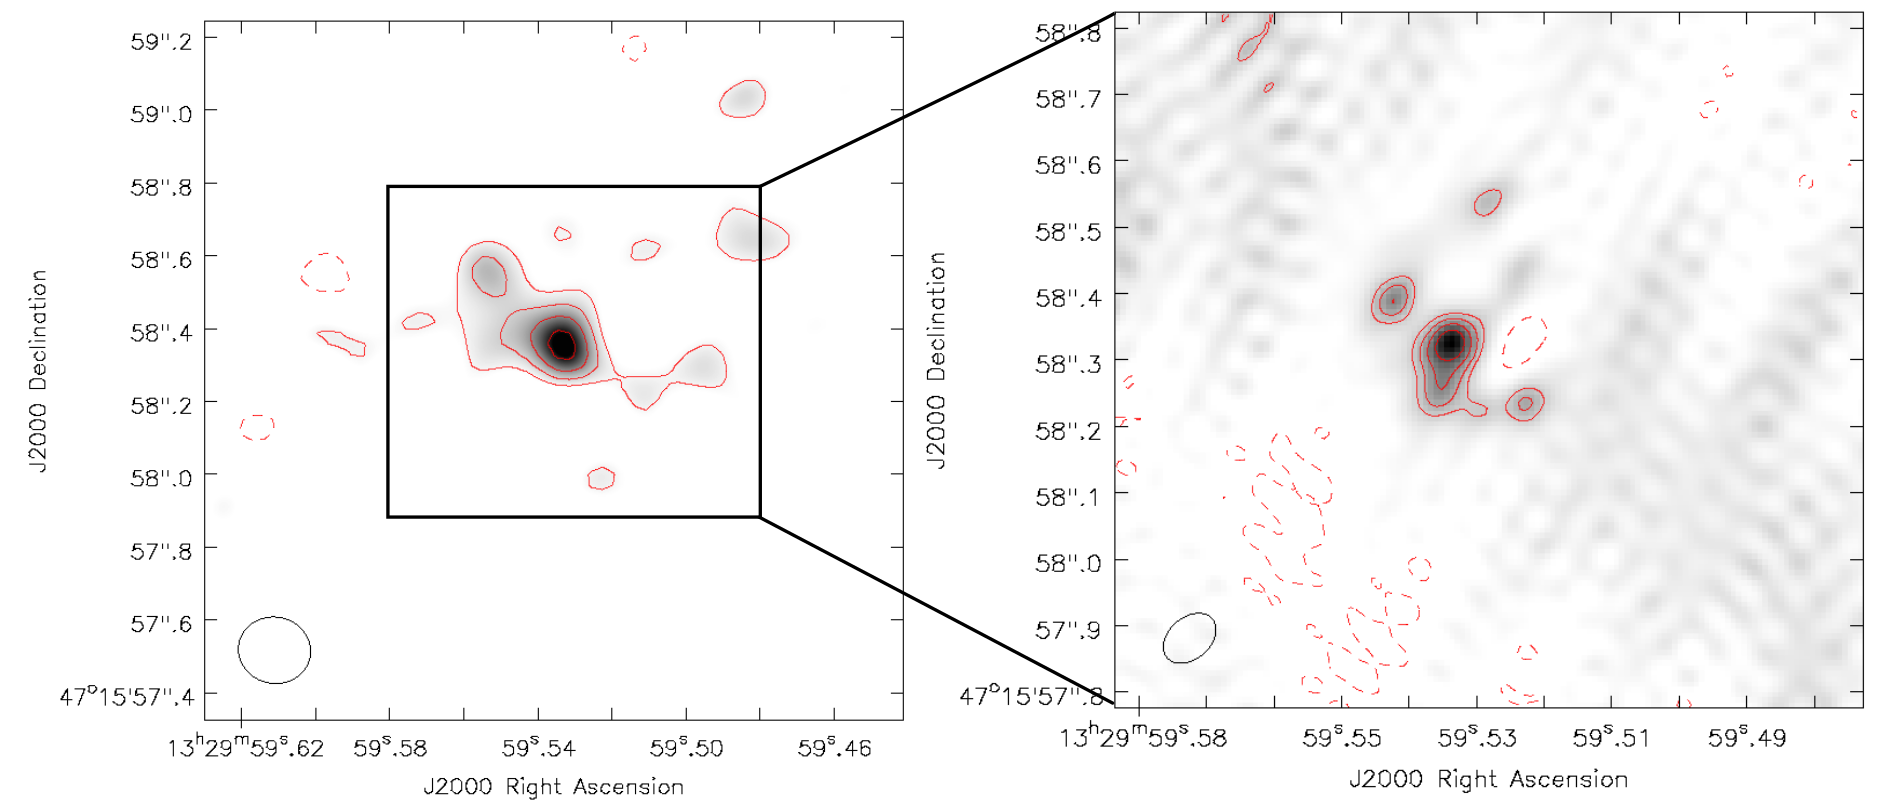
\includegraphics[scale=0.5,clip=true,trim=0cm 0.1cm 0cm 0cm]{eMERLIN_combine_image.png}
\caption{e-MERLIN maps of the nuclear region of NGC~5195. The image on the left plots the 1.4 GHz e-MERLIN contours and the right plots the e-MERLIN 5.0 GHz contours overlayed on the respective greyscale images. The contours are at -3,3,4,5,6,7 $\times~\sigma_{rms}$ given in \tab~\ref{tab:fluxMeas}. The images display a partially resolved source with possible parsec-scale  outflow. Negative contours are dashed. The synthesized beam sizes for both images are listed in \tab~\ref{tab:fluxMeas}.} 
\label{fig:MERLINimg}
\end{figure*}
%------------------------------------------



\subsection{Archival VLA - Continuum} 
\label{sec:vla_cont}
We make use of archival multi-configuration VLA observations centred on NGC~5194 at \textbf{1.4, 4.9 and 8.4 GHz}, which 
are summarised in \Tab~\ref{tab:vlaObs}. The calibration procedures are explained in detail by 
\cite{Dumasetal2011}. Prior to imaging, the datasets were averaged in time and frequency to minimise 
amplitude losses due image smearing to less than 1~$\%$ at the edge of the primary beam. \textbf{For 
each frequency, the uv datasets for the different configurations were combined within \textsc{casa} 
and imaged using multi-scale clean \citep{RC2011}, with scales at 0, 5, 10 and 15 pixels. }For 
accurate morphological and flux density comparisons, the final images (at each frequency) were made 
with minimum and maximum uv-range of 0.5~k$\lambda$ and 180~k$\lambda$ respectively, cellsize of 
0.23\arcs, and robust 1 weighting. Since the datasets were all centred on NGC~5194, to include 
NGC~5195 ($\approx$~5\arcm offset), wide-field images of radius 12\arcm were made \textbf{using the 
w-projection \citep{wproj} with 128 planes}.  Primary beam effects were \textbf{corrected via} the 
\textsc{casa} task \textsc{impbcor}, and finally a sub-image of NGC~5195 was extracted using 
IMSUBIMAGE. The final images are shown in \fig~\ref{fig:VLAMaps} \textbf{and \tab~\ref{tab:fluxMeas} 
lists the flux densities for the unresolved radio core obtained using the \textsc{casa} task 
\textsc{imfit} and listed in \tab~\ref{tab:fluxMeas}. The uncertainty in the final flux density 
measurements are affected by three main sources: (1) fitting errors from \textsc{imfit}, (2) a 
fiducial flux calibration error of $5\%$, (3) the image rms (listed in \tab~\ref{tab:fluxMeas}). All 
three are added in quadrature and adopted as the error measurements in \tab~\ref{tab:fluxMeas}.}  



\begin{center}
\begin{table}\footnotesize
\caption{\textsc{Archival VLA Observations}}
\label{tab:vlaObs}
\hfill{}
\tabcolsep=0.11cm
\begin{tabular}{lcccc}
\hline\hline
\noalign{\smallskip}
Band & Config & $\nu$ &    Date     & Time \\ 
     &               & (GHz) &   & (h) \\ 
(1)  &      (2)      & (3)   &   (4)       &  (5)   \\ 
 \hline 
L & A & 1.385$^{*}$;1.465$^{*}$ & 10/2004 & 30.8 \\
  & B & 1.385$^{*}$;1.465$^{*}$ & 06/2005   & 23.9 \\
  & C & 1.465$^{\dagger}$ & 04/1992  & 13.4 \\
  & D & 1.465$^{\dagger}$ & 07/1988 & 12 \\
\hline
C & B & 4.876$^{*}$ & 12/2003-03/2005 & 23 \\
  & C & 4.835$^{\dagger}$ & 07/2001 & 14.4 \\
  & D & 4.885$^{\dagger}$ & 03-04/1991 & 8.7 \\
\hline
X & C & 8.435$^{\dagger}$ & 04/2005 & 20.3 \\
  & D & 8.435$^{\dagger}$ & 10-11/2001 & 17.6 \\
\hline
\hline
\multicolumn{5}{l}{\textbf{Notes.} See \citealt{Dumasetal2011}, \tab~2 for more details. }\\
\multicolumn{5}{l}{$^{\dagger}$ bandwidth = 50 MHz; $^{*}$ bandwidth = 25 MHz }\\
\multicolumn{5}{l}{\textit{Columns:}(1) Band name; (2) VLA configuration; }\\
\multicolumn{5}{l}{(3) Central observing frequency for each IF; (4) Observing}\\
\multicolumn{5}{l}{dates (mm/yy); (5) Total on-source integration time}

\end{tabular}
\hfill{}
\end{table}
\end{center}



\begin{center}
\begin{table*}\footnotesize
\caption{\textsc{Radio Interferometric Measurements of NGC~5195}}
\label{tab:fluxMeas}
\hfill{}
\begin{tabular}{lccccccc}
\hline\hline
\noalign{\smallskip}
Array & $\nu$ & $S_{pk}$ & $S_{int}$ & log($L_{\nu}$/WHz$^{-1}$) & $\sigma_{rms}$ & $\Theta_{beam}$  & P.A.\\ 
      & (GHz) & (\mjybm) & (mJy)	 &  & \mujybm & (\arcs $\times$ \arcs)  & (\deg)\\ 
(1)   & (2)   &  (3) 	& (4) 		 & (5)  & (6) & (7) & (8)\\ 
 \hline 
%MERLIN  & 1.66 & 0.42 $\pm$ 0.06 & 1.67 $\pm$ 0.03 & 19.15 & 61.70 & 0.22 $\times$ 0.17 & -29 \\
e-MERLIN$$ & 1.51 & 0.47 $\pm$ 0.09 & 3.00 $\pm$ 0.06 & 19.40 & 98.90 & 0.20 $\times$ 0.18 & 79 \\
%e-MERLIN & 1.510 & 0.464 $\pm$ 0.056 & 1.113 $\pm$ 0.018 & & 0.27 $\times$ 0.15 & -67 \\
e-MERLIN$$ & 5.07 & 0.16 $\pm$ 0.03 & 0.50 $\pm$ 0.11 & 18.63 & 26.90 & 0.09 $\times$ 0.06 & -49 \\
\hline
VLA$^{\dagger}$ & 1.43 & 4.55 $\pm$ 0.11 & 6.27 $\pm$ 0.24 & 19.68 & 24.42 & 4.01 $\times$ 3.45 & -79\\
VLA$^{\dagger}$ & 4.86 & 2.12 $\pm$ 0.04 & 2.79 $\pm$ 0.09 & 19.33 & 14.13 & 4.01 $\times$ 3.45 & -79\\
VLA$^{\dagger}$ & 8.44 & 1.57 $\pm$ 0.03 & 1.90 $\pm$ 0.05 & 19.16 & 11.56 & 4.01 $\times$ 3.45 & -79 \\
\hline
\hline
\multicolumn{8}{l}{\textbf{Notes.}}\\
\multicolumn{8}{l}{$^{\dagger}$ Nucleus only. \textit{Columns:}(1) Array; (2) Central Frequency; (3) Peak flux density; (4) Integrated flux density;}\\
\multicolumn{8}{l}{(5) Luminosity in logscale of column (4) ; (6) Image noise;  (7- 8) Beam size and beam PA}
%\multicolumn{8}{l}{}

\end{tabular}
\hfill{}
\end{table*}
\end{center}


\begin{figure*}\scriptsize
\centering
\subfloat[L~Band]{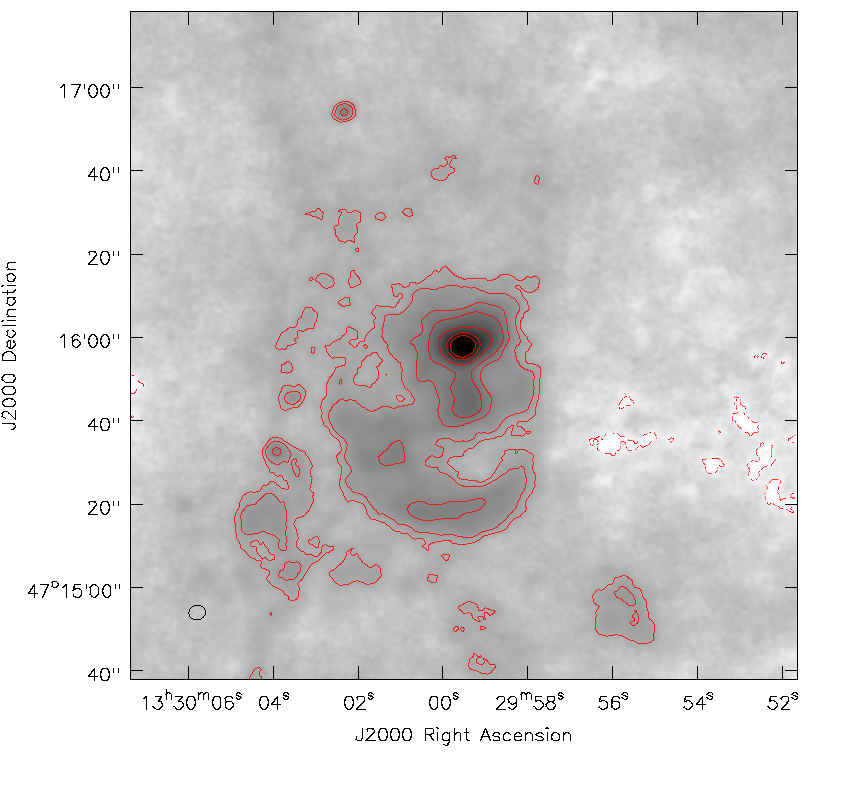
\includegraphics[scale=0.43,clip=true,trim=0cm 2cm 1cm 0cm]{M51b_20cm_gscale_cp.png}}
\subfloat[C~Band]{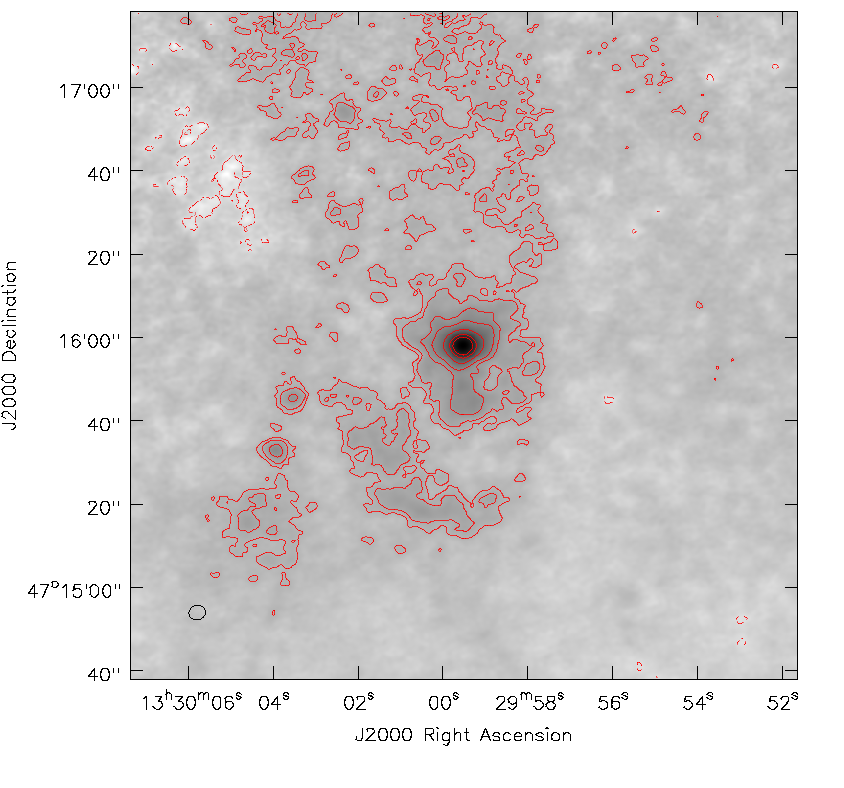
\includegraphics[scale=0.43,clip=true,trim=0cm 2cm 1cm 0cm]{M51b_6cm_gscale.png}}\\
\subfloat[X~Band]{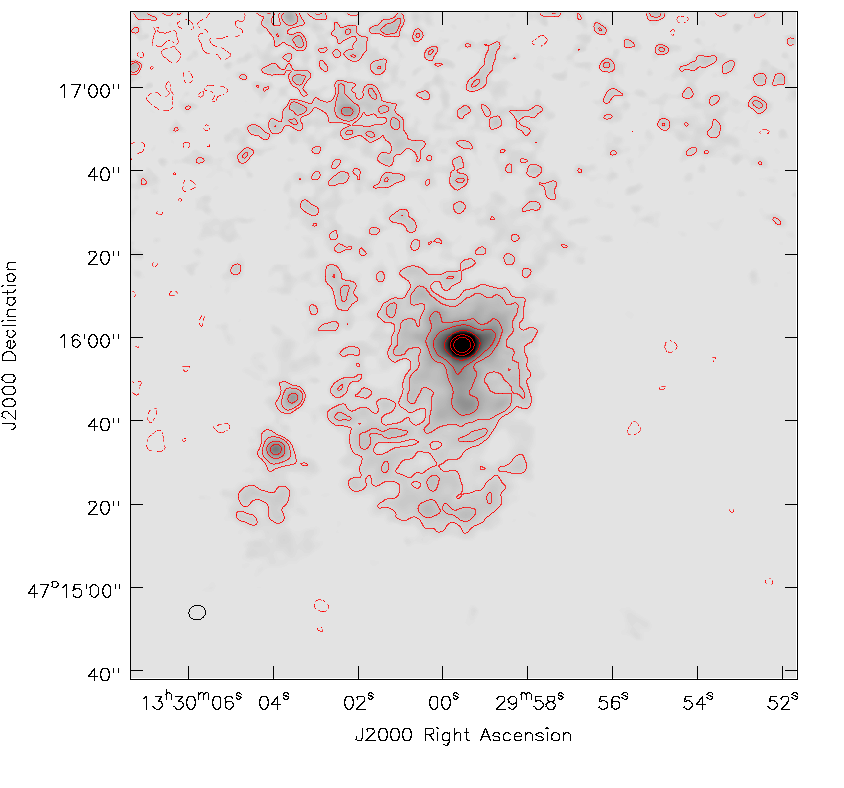
\includegraphics[scale=0.43,clip=true,trim=0cm 2cm 1cm 0cm]{M51b_3cm_gscale.png}}
\caption{Multi-scale, multi-configuration, multi-frequency VLA images of NGC~5195. The peak fluxes and the image noise, $\sigma_{rms}$ are given in \tab~\ref{tab:fluxMeas}. The contours in each image are (-3, 3, 5, 10, 15, 30, 60, 90) $\times\, \sigma_{rms}$. Present in all three images are the core, an elongated structure south of the core (hereafter ``jet") and an arc-like emission south of the jet and core. Negative contours are dashed. The synthesized beam sizes for both images are listed in \tab~\ref{tab:fluxMeas}.}
\label{fig:VLAMaps}
\end{figure*}


\subsection{Multi-Wavelength Data}

Optical images of the M51 system were acquired from the Hubble Space Telescope (HST) online archive by \cite{Rampadarathetal15}. For this study we used the images taken with the Advanced Camera for Surveys (ACS)\footnote{\textit{HST} observing program 10452, P.I. Steven V. W. Beckwith.} \textit{F658N} filter that have been continuum-subtracted showing only H$\alpha$ + [N~II] emission lines.

\textbf{Similarly, the M51 system has been observed 12 times  (considering only observations longer than 2 ks) with the \textit{Chandra}/ACIS-S X-ray telescope between 2000 and 2012 (see Table 3 of \citealt{Rampadarathetal15}). The datasets were downloaded from the public Chandra archive. Each observation was reprocessed using tools available in CIAO version 4.5 CITE and CALDB version 4.5.3, to obtain new level-2 event files. The event files were reprojected to a common point and combined, to obtain an image of the M51 system which is described in detail by \cite{Rampadarathetal15}.}

%\section{Discussion}  - boring ;-)
%\section{Exploring the nucleus}
\section{the radio structure of ngc~5195}

\subsection{Sub-arsecond scale emission}
%Description of what we see in the new e-MERLIN data.

\Fig~ \ref{fig:MERLINimg} shows the e-MERLIN images of NGC~5195 at both 1.5 and  and 5.1 GHz. The images reveal a partially resolved compact radio source, with faint extended emission with an elongated morphology, possibly outflows from the AGN. High resolution radio studies using e-MERLIN and VLBI have shown that outflows/jets are common in nearby low-luminosity AGN (e.g. \citealt{Krips+2007,GP09}). While the MERLIN/e-MERLIN images do suggest a similar core-outflow/jet structure, obtaining a spectral index map would provide more certainty. However, large differences in the uv-coverage, combined with the low signal-to-noise ratio of the emission (3-5$\sigma_{rms}$), made it difficult to combine the datasets to determine the spectral index distribution with any degree of confidence. 

A recent survey of the M51 system with the European 
VLBI Network (EVN) at 18~cm ($B_{maj} \approx 10$~mas) failed to detect any emission arising from the 
NGC~5195 core above a limit of 132~\mujybm~ \citep{Rampadarathetal15}. This places an upper limit on 
the power output of the AGN core of $\approx\,10^{18}\,{\rm W\,Hz^{-1}}$ ($10^{34}\,{\rm 
erg\,s^{-1}}$) and the brightness temperature ${\rm T_{B}}\leq\,9\,\times\,10^{5}$~K. Thus suggesting 
that the sub-arcsecond radio emission is dominated by extended emission such as outflows and star-formation \citep{Padovani2016}.



%-------------------------------------------
\begin{figure*}
{\centering
\subfloat[X~rays]{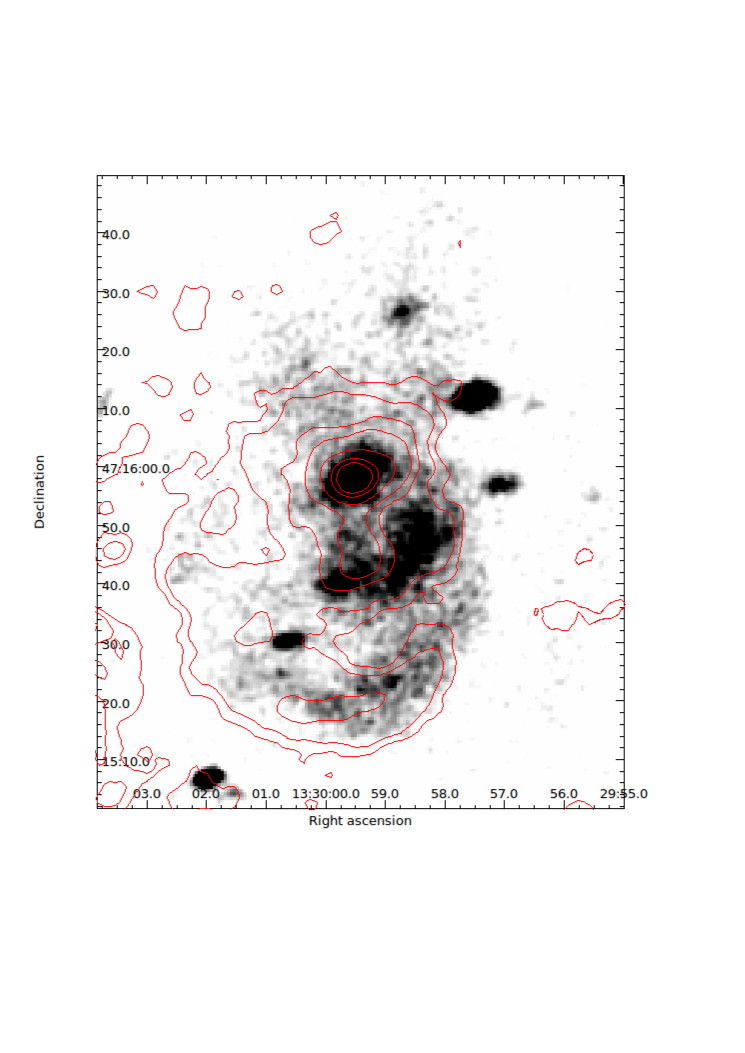
\includegraphics[scale=0.35,clip=true,trim=1cm 6.8cm 1cm 2cm]{radio_xray_2.png}} \hspace{2em}
\subfloat[H$\alpha$]{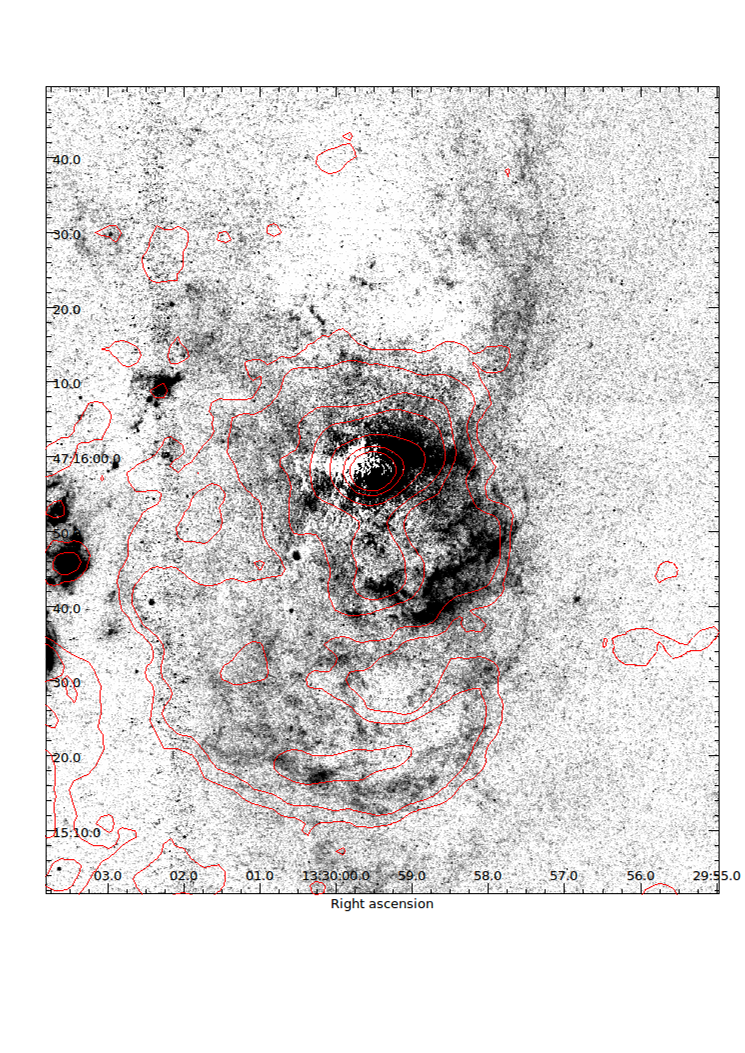
\includegraphics[scale=0.28,clip=true,trim=1cm 4cm 0cm 3cm]{radio_halpha_2.png}}\\
\subfloat[Radio, X-rays and H$\alpha$]{\includegraphics[scale=0.11,clip=true,trim=30cm 15cm 60cm 10cm]{M51b_rgb_cube.png}}

\caption{(a): \textit{Chandra}/ACIS-S X-ray image of NGC~5195 at 0.3 - 2 keV. (b): \textit{HST}/ACS continuum-subtracted image in the \textit{F658N} filter (H$\alpha$) of the same field. Both are overlayed with VLA multi-configuration L-band contours from \fig~\ref{fig:VLAMaps}a. (c): false colour rgb image made by combining the 20 cm VLA radio image (red) with the \textit{Chandra} X-ray image (green) and the \textit{HST} H$\alpha$ image (blue). The images show strong agreement in morphology across all three frequencies.}
\label{fig:VLAHalpha}
}
\end{figure*}
%------------------------------------------


\subsection{Arcsecond scale emission }

The VLA images (Figure \ref{fig:VLAMaps}) reveal a number of interesting features: (1) a bright compact source at the galaxy's centre containing the AGN and e-MERLIN source; (2) an ejecta or jet-like emission, that extends 15\arcs ($\approx$ 0.6 kpc) south of the nucleus (hereafter referred to as ``jet"); (3) an arc of emission 20\arcs - 40\arcs ($\approx$ 0.8 - 1.6 kpc) south of the nucleus, that appears to curve around the jet and nucleus (hereafter referred to as ``radio-arc"). 

\textbf{Interestingly, the jet lacks hot spots that generally demarcates the end of the jet found in more powerful AGNs (e.g. \citealt{PT2000,Girolettietal2003}). This suggests a relatively low velocity jet ($\beta~<~0.76$) that is unable to bore through the local ISM and escape \citep{GGT2004}.
}

There is evidence for diffuse, low-surface brightness emission to the North of NGC~5195, that appears 
to extend out of the nucleus. It is difficult to say with confidence whether this is real emission as 
the structure is not consistent across all frequencies. In addition, the distance of NGC~5195 from the pointing centre of the VLA observations (i.e. at the outer edges of the primary beam) increases the image rms noise and hence the uncertainty of the emission being real.

The study by SJMV reported the detection of a pair of X-ray and H$\alpha$ arcs, one at 15\arcs (the ``inner arc") from the nucleus, and  another at $\sim$ 30\arcs (the ``outer arc"). \Figs~\ref{fig:VLAHalpha}a $\&$ b show the \textit{Chandra}/ACIS-S image at 0.3 - 2 keV and \textit{HST}/ACS continuum-
subtracted H$\alpha$ images, with the radio contours from \fig~\ref{fig:VLAMaps}a overlayed.
In both images, the radio jet terminates in regions of bright X-ray and H$\alpha$ emission, with only the 
most southern part of the radio-arc corresponding to X-ray and H$\alpha$ emission. This is most evident in 
the RGB-combined image in \Fig~\ref{fig:VLAHalpha}c. T\textbf{he images also show the H$\alpha$ emission in the outer arc appears to lie on the outer edge of the X-ray arc. SJMV suggested that this is evidence for displacement of H$\alpha$-emitting material from the core by the X-ray-emitting gas}. 

\textbf{However, It is also possible that the mechanism responsible for accelerating the electrons and producing the 
radio emission, is also responsible for the X-ray and the H$\alpha$ emission. This will be explored in \sects~\ref{sec:jet_pwr} and \ref{sec:xrays_orign}.}


\subsection{Spectral index}

To further understand the nature of the emission, the L-, C-, and X-band images were combined to create a spectral index map. Since the VLA data have already been imaged using the same uvtaper, cellsize and weighting parameters, the C- and X-band images were re-gridded (via the AIPS task REGRD) to match the L-band image. The three images were 
exported as FITS files and, using astropy, numpy and scipy.optimize.curve$\_$fit, we computed the spectral index map shown in \fig~\ref{fig:Specind}. To remove biasing to steep $\alpha$ values due to noise and negative pixels, a 1$\sigma$ flux density cut was imposed on the three images, where $\sigma$ is the rms noise of each uvtapered image\footnote{The choice of a 1$\sigma$ cut was chosen since the arc is detected at the 3-5 $\sigma$ level in the 1.4 GHz image but barely so in the higher frequencies. Thus the spectral index in the arc should be taken as an upper limit.}. The final spectral index and noise maps are shown in \fig~\ref{fig:Specind}. 

\textbf{The spectral index obtained for the core and jet ($\alpha \approx$ -0.6 to -0.7) are as expected for a jet with plasma that is being accelerated from the base of the jet \citep{NWF01}. However, spectral index is significantly steeper within the arc ($\alpha <$ -0.7). This steepening of the spectral index in the arc can be the result of synchrotron ageing \citep{CPDL91}, or energy losses due to adiabatic expansion of the material as it does work on its surroundings \citep{CPDL91}. Higher sampling of the radio spectrum at lower radio frequencies are required for full analysis of either effects, and is beyond the scope of this paper.}

%-------------------------------------------
\begin{figure*}
{\centering
\subfloat[Spectral index map]{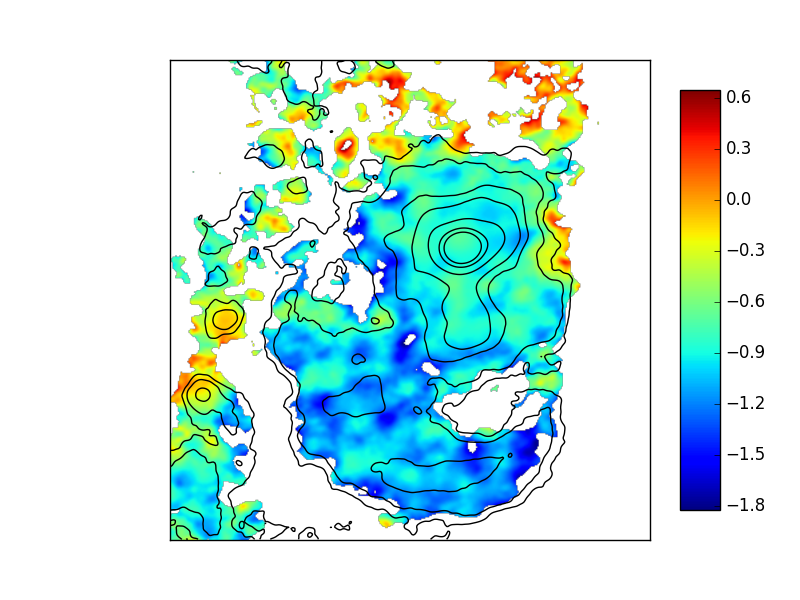
\includegraphics[scale=0.45,clip=true,trim=3cm 1cm 0.5cm 1.5cm]{VLA_SPECIND.png}} \hspace{2em}
\subfloat[Error map]{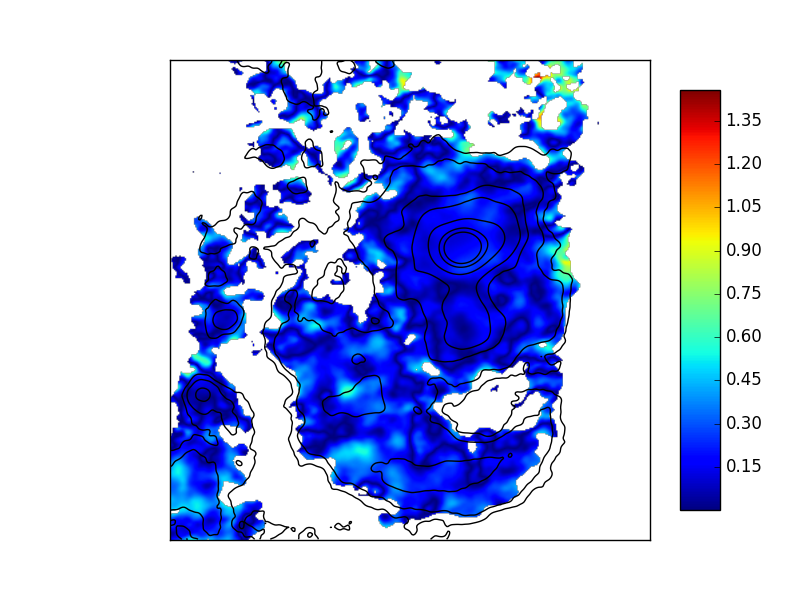
\includegraphics[scale=0.45,clip=true,trim=3cm 1cm 0.5cm 1.5cm]{VLA_SPECIND_err.png}}

\caption{Spectral index map (left) and the corresponding error map (right) of NGC~5195, obtained through combining the VLA L, C and X band images. Overlayed are the VLA L-band contours from \fig~\ref{fig:VLAMaps}a. The spectra index gradually increases outwards from the core towards the radio-arc.}
\label{fig:Specind}
}
\end{figure*}
%------------------------------------------

% This is a large sub-section, split it out into its own section?
\section{Is the jet responsible for the arcs/bubbles?}
\label{sec:jet_pwr}

\textbf{In this study, we show the existence of a sub-kpc outflow coincident with X-ray and H$\alpha$ arcs. It is possible that the mechanism responsible for accelerating the electrons to create the radio emission is responsible for both the X-ray and H$\alpha$ emission. If this is true, then one would expect the power output of the nucleus and jet would be sufficient to inflate the X-ray and H$\alpha$ bubble. }To determine this, we estimate the jet power and compare it to the power required to inflate the bubbles.

\textbf{The relationship between AGN jet power and observed radio luminosities is an active field of 
research. There have been a number of studies suggesting relationships between the core an lobe 
luminosities with the jet power (see \citealt{MH07,BF2011,GS2016} and references therein). We 
estimate the kinematic jet power from the core radio luminosity at 5~GHz, $L_{5 \rm GHz}$, using the 
relation by \cite{MH07}: $L_{\rm kin} = (0.81\,\pm\,0.11)\,{\rm log}L_{5 \rm GHz}\, +\, 
11.9^{+4.1}_{-4.4}$.} From the integrated flux density listed in \tab~\ref{tab:fluxMeas}, we obtain 
$L_{5 \rm GHz} = 1.07 \pm 0.04 \times 10^{36} {\rm erg~s^{-1}}$ and from the relation above, $L_{\rm 
kin} = 1.21^{+0.62}_{-0.66} \times 10^{41} {\rm erg~s^{-1}}$. 

Optical line emission from shocked gas (e.g. H$\beta$), is a reliable measure for mechanical power, 
such as from jets (e.g. \citealt{DopitaSutherland1996,Allenetal2008}). Standard bubble theory \citep{Weaver+1977} predicts for a fully radiative shock expanding into the ISM, \textbf{$L_{\rm rad} \approx (27/77)L_{kin}$, where  $L_{\rm rad}$ is the radiative power and $L_{\rm kin}$, the mechanical power.}
This amount of energy is mostly radiated in the form of IR/optical/UV lines. Radiative shock models ({\it e.g.}, 
{\small {MAPPINGS III}}: \citealt{DopitaSutherland1996}, \citealt{Allenetal2008}) are then used to 
predict the flux distribution between the main lines as a function of shock velocity and ISM density. 
For typical densities ($\sim$0.1--10 cm$^{-3}$), shock velocities between 100 and 500 km s$^{-1}$, 
solar metallicity and equipartition magnetic field\footnote{\textbf{In MAPPINGS III the magnetic field, $B$ and magnetic parameter are chosen to cover extremes expected in the interstellar medium, 
while finely sampling magnetic field strengths near equipartition. Under equipartition conditions the magnetic 
pressure is equal to the thermal pressure, which occurs when $B$ = 3.23 $\mu$G, for a pre-shock 
density of 1~cm$^{-3}$. See \citealt{Allenetal2008} for details.}}, \textbf{H$\beta$ emission accounts for a 
fraction $\approx\, 6.5\, \pm\, 1.5\, \times\, 10^{-3}$ of the radiative output power, which gives  $L_{\rm{H}\beta} \approx\, 2.2\, \pm\, 0.5\, \times\, 10^{-3} L_{\rm kin}$, where $L_{\rm{H}\beta}$ is the H$\beta$ luminosity.} Thus, H$\beta$ luminosity is a powerful diagnostic line for the 
jet power \citep{Pakull+2010}. We do not have a direct measurement of H$\beta$ in NGC 5195; however, 
we can take the measured (and de-reddened) H$\alpha$ flux and assume $F_{{\rm{H}}\alpha} \approx 
2.86F_{{\rm{H}}\beta}$ \citep{OF2006}.

To this end, we measured the background-subtracted count rate in the inner and outer arcs from the 
{\it HST}/ACS image in the F658N filter, which includes H$\alpha$, [N II] $\lambda$ 6548, and [N II] 
$\lambda$ 6583. We multiplied the count rate by the flux-density normalization value PHOTFLAM, and then 
multiplied by the effective width of the filter, to obtain the combined flux in the lines covered by 
the filter. The effective width of F658N is listed as 78 \AA\ in Table 5.1 of the ACS Instrument 
Handbook \footnote{\url{http://www.stsci.edu/hst/acs/documents/handbooks/current/c05_imaging2.html}}. We 
checked this value using the python task {\small{PYSYNPHOT}}\footnote{\url{https://pysynphot.readthedocs.io/en/latest/index.html}} (as recommended by Jenna Ryon, ACS Instrument Team, priv.~comm.), under the 
plausible assumption that the three lines are much narrower than the filter width. We obtained an 
effective bandpass of 75 \AA\ with {\small{PYSYNPHOT}}, which is the value we adopt here. Thus, the 
total de-reddened flux in the F658N filter is $F_{\rm{F658N}} \approx 3.2 \pm 0.2 \times 10^{-13}$ erg~s$^{-1}$~cm$^{-2}$.

The next step is to estimate what fraction of the flux in the F658N filter belongs to H$\alpha$ and 
what fraction to the two [N II] lines. This ratio is again a function of ISM density, metallicity, and 
shock velocity \citep{Allenetal2008}. Observations by \cite{Hoopes-Walterbos} suggest a ratio of [N II] 
$\lambda$ 6583/H$\alpha$ $\approx 1.3$ in our region of interest (see their Table 5 and Fig.~19). When 
the expected contribution from [N II] $\lambda$ 6548 is also taken into account (with a theoretically 
predicted value of $F_{6583} \approx 2.95 F_{6548}$, almost independent of ISM conditions: \citep{Allenetal2008}, we obtain that $F_{{\rm{H}}\alpha} \approx
0.37F_{\rm{F658N}}$. Finally, we estimate $F_{{\rm{H}}\beta} \approx 0.35F_{{\rm{H}}\alpha} \approx 
0.13F_{\rm{F658N}}$. We obtain $F_{{\rm{H}}\beta} \approx 4.2 \times 10^{-14}$ erg~s$^{-1}$~cm$^{-2}$. At the assumed distance of 8~Mpc, this corresponds to a luminosity $L_{\rm{H}\beta} \approx 3.2 \pm 0.12
\times 10^{38}$ erg~s$^{-1}$. Thus the mechanical power required to inflate the H$\alpha$ bubble in NGC~5195 is $L_{\rm kin} \approx 1.45 \pm 0.24 \times 10^{41}$ erg~s$^{-1}$
However, this is only the estimate for the southern component of the jet. 
We must assume that there is also a northern component with the same power, even though the ISM density 
there is too low to produce substantial line emission. Thus, the total mechanical power required to inflate the observed H$\alpha$ bubble, inferred from 
the Balmer lines is $L_{\rm kin} \approx 2.9 \pm 0.24 \times 10^{41}$ erg~s$^{-1}$. 

\textbf{The factor of 2 difference in both values for $L_{kin}$ reflects the uncertainty in the calculations 
presented here. In using the optical emission, there were a number of assumptions whose uncertainty is difficult to estimate. One such is that all H$\alpha$ emission are shock generated. While the line ratios presented by \cite{Hoopes-Walterbos} in the region of the H$\alpha$ bubble strongly favours shock ionisation, \cite{Alataloetal2016} showed that NGC~5195 is efficiently forming stars, suggesting possible contamination from star-formation.}

\textbf{Furthermore, the use of radio luminosity to estimate the jet power is in itself uncertain. Aside from the small sample size of \cite{MH07}, and the large scatter, \cite{GS2016} 
argued that such studies of the scaling relations between radio luminosities and jet power in 
powerful radio galaxies (i.e. Fanaroff-Riley types I and II, \citealt{FR74}) are affected by 
distance. They furthermore suggest that this correlation with lobe luminosity may
be weak when the jet energy is dissipated along its path, for example by driving shocks. Nonetheless, 
considering the calculation of the jet power using different methods (radio power vs. optical line 
emission) agree within a factor of two is encouraging and suggests a similar origin of the H$\alpha$ and 
radio emission within NGC~5195.}

 %Which is in good agreement with the estimation of $L_{\rm kin}$ using the radio core flux density, considering the systematic uncertainties in both relations.

%\subsection{The origin of the X-ray emission}
\section{The origin of the X-ray emission}
\label{sec:xrays_orign}

SJMV suggest that the curvatures of the X-ray arcs argue for a nuclear origin, at or near the SMBH. In this 
scenario, the arcs are signatures of periodic outbursts arising from infalling matter onto the SMBH 
resulting from a recent merger of the galaxy pair. However, it is possible that the X-ray emission is due 
to other sources within the nuclear region of NGC~5195. 
For example, observations of the interacting starburst system NGC~7714/7715 with \textit{Chandra} by 
\cite{SSN2005} detected an unresolved variable X-ray source within the nucleus. They suggested the X-ray 
emission is possibly from supernovae, O-type stars, Wolf Rayet (W-R) stars,
hot gas, high-mass X-ray binaries (HMXBs), or ULXs. Based upon the lack of evidence for an AGN from 
infrared spectra and an estimated SMBH mass of $< 10^{5}$ M$_{\odot}$, they ruled out an AGN as the source 
or main contributor. While we are certain of the existence of an AGN in NGC~5195, there is a possibility 
that some or all of the X-ray emission may have arisen from another source. 

\textbf{According to the fundamental plane of black hole activity (e.g. \citealt{Merloni+2003,Falcke+2004,Kordingetal2006b}) the radio, X-ray luminosities and black hole masses shows correlations from stellar mass black holes to the SMBH within AGNs. The general picture is one whereby the emission from the jet and/or disc of an active black hole are connected, thereby producing the observed correlations, defined as $\log L_{\rm R}\,=\,(4.80\,\pm\,0.24)\,+\,(0.78\,\pm\,0.27)\log M_{\rm BH}\,+\,(0.67\,\pm\,0.12)\log L_{\rm X}$ \citep{Gultekinetal2009}, where the X-ray luminosity refers to the 0.5--10 keV band and $L_{\rm R}$ the radio luminosity at 5~GHz.}

The mass of the SMBH can be estimated from the $M$-$\sigma$ relation \citep{vandenBosch2016}. Specifically, we used the velocity dispersion $\sigma \approx 127.4\,\pm\,4.9$ km s$^{-1}$ from the Hyperleda database\footnote{\url{http://leda.univ-lyon1.fr/}} and obtained a best-fitting mass $M \approx 10^{(7.27\pm 0.33)} M_{\odot}$. While we use $L_{\rm R} \approx 1.07 \pm 0.04 \times 10^{36}$ erg s$^{-1}$ given in \sect~\ref{sec:jet_pwr}. Thus, the expected X-ray luminosity from the Fundamental Plane, $L_{\rm X} \approx 1.40 \pm 0.86 \times 10^{39}$ erg s$^{-1}$. 

On the other hand, the unabsorbed X-ray luminosity we determined from our spectral modelling of the 
{\it Chandra} X-ray spectrum is $L_{\rm X} (0.3$--$10.0 keV) \approx 0.8 \pm 0.13 \times 10^{39}$ erg s$^{-1}$ at the assumed 
distance. This value includes only the power-law component of the X-ray spectrum (photon index $\Gamma 
\approx 1.56$), which is likely to be directly attributable to the nuclear SMBH. An additional 
(spatially unresolved) thermal-plasma component at a characteristic temperature $kT \approx 0.3$ keV 
contributes a thermal (mekal\footnote{mekal is a standard emission model available in CIAO and is an emission spectrum from hot diffuse gas from several elements.  Please see \url{http://cxc.harvard.edu/sherpa/ahelp/xsmekal.html} for details.}) luminosity, $L_{\rm{mekal}} \approx 0.8 \pm 0.13 \times 10^{39}$ erg s$^{-1}$: this may be evidence 
of a compact star-forming nucleus, or of gas shock-ionized by the nuclear jet, \textbf{or thermal wind from the accretion disk}. Considering the 
intrinsic scatter in both the $M$-$\sigma$ relation and the fundamental plane, we conclude that the 
predicted and observed luminosities of the nuclear SMBH are in good agreement at $L_{\rm X} \approx 
10^{39}$ erg s$^{-1}$. The bolometric luminosity can be estimated as  $L_{\rm {bol}} \sim$ \textbf{16} $L_{\rm X}$ 
\citep{Ho2008}, hence $L_{\rm {bol}} \sim 1.6 \times 10^{40}$ 
erg s$^{-1}$. Therefore, the Eddington ratio $L_{\rm{bol}}/L_{\rm{Edd}} \approx$ a few $10^{-6}$, 
falling in the radiatively-inefficient regime.

\textbf{We now determine the radio loudness of NGC~5195 using the relation defined by \cite{TW2003} as $R_{X} \equiv L_{\nu}(5 ~\rm GHz)/L(2-10~ \rm keV)$. From the \textit{Chandra} data we obtain $L(2-10~ \rm keV) = 0.51 \pm 0.09 \times 10^{39}$ from our spectral modelling. With $L_{\nu}(5 ~\rm GHz) = 1.07 \pm 0.04 \times 10^{36}$ erg s$^{-1}$, we get log$_{10}(R_{X})$ = -2.7 which places NGC~5195 on the border between low-luminosity radio galaxies and LLAGNs (see \figs~5 and 7 of \citealt{Panessaetal2007}). 
}

\section{Conclusion}

\textbf{Our results support the idea that the mechanism responsible for the radio emission, is driving 
the X-ray and H$\alpha$ arcs. Where the recovered spectral index, favours a non-thermal origin of the 
radio emission, thus, generating the X-ray and H$\alpha$ emission via shocks. This is consistent with 
the optical line spectra \citep{Hoopes-Walterbos}, which show emission from shock-ionized gas. 
However, this contradicts the assertion from \cite{Alataloetal2016} that all radio emission present 
within the vicinity of NGC5195's nucleus, is most likely associated with star-formation rather than AGN 
activity. The results of \cite{Kohnoetal2002} indicates that NGC~5195 is in a post-starburst stage with 
the high stability of the remaining diffuse molecular gas unable to form dense cores via gravitational 
instabilities. Thus, while we cannot rule out contributions from star-formation, we are confident from 
that analysis presented in this study, that it is not the dominant contributor to the radio emission at 
centimetre wavelengths.} 



\section{Summary}

We present a detailed study of the nearby irregular galaxy NGC~5195, making use of new e-MERLIN, 
observations and archive VLA data, X-ray images from \textit{Chandra} and H$\alpha$ images from 
\textit{HST}. Below, we summarise the main findings of this study:

\begin{enumerate}
\item With the VLA, the radio emission from NGC~5195 on scales of a few hundred parsecs is divided into an unresolved radio core, an ejecta/outflow or jet, and a radio-arc;
\item The e-MERLIN observations reveal a partially resolved source with faint extended emission, possibly outflows from the AGN;
% \item Using previous VLBI observations we place an upper limit on 
% the power output of the AGN core of $\approx\,10^{18}\,{\rm W\,Hz^{-1}}$ ($10^{34}\,{\rm 
% erg\,s^{-1}}$) and the brightness temperature ${\rm T_{B}}\leq\,9\,\times\,10^{5}$~K.
\item The morphology of the VLA jet and radio-arc corresponds to arcs (or bubbles), previously detected in the X-rays with \textit{Chandra} and H$\alpha$ with \textit{HST};
\textbf{\item The spectral index distribution of the core and jet are typical for a jet with plasma accelerated at the base of the jet. While the radio-arc possesses a steeper spectrum, possibly from spectral ageing or adiabatic expansion;}
\item Comparing the energetics, we demonstrate that the recent power output of the radio jet is sufficient to generate the H$\alpha$ arcs and filaments, based on standard models of optical line emission from shock-ionized gas. In other words, such features do not require NGC~5195 to have experienced much higher bursts of nuclear activity in the past few Myr;
\item Taking the compact radio core luminosity at 5~GHz, the power-law component of the {\it Chandra} nuclear source as the X-ray core luminosity,\textbf{ and an estimate of the black hole mass from the M - $\sigma$ relation,} we show that the SMBH \textbf{is within the estimates of} the fundamental plane, with an Eddington ratio $\sim$ a few $10^{-6}$;
\textbf{\item The radio-loudness and Eddington ratio places NGC~5195 in the region between the brightest LLAGNs and the faintest low-luminosity radio galaxies.}

\end{enumerate}

\textbf{The radio emission in NGC~5195 shows diverse properties. It's dominated by extended outflows, while possessing a very faint compact core. Further observations of NGC~5195 are required: (i) to reveal the exact nature of the radio emission with deep polarisation studies with the Jansky VLA, (ii) high sensitive multi-wavelength e-MERLIN observations to explore the extended outflows, (iii) being able to detect the VLBI core will be a great opportunity to study the emission process of a nearby faint-AGN on sub-parsec scales, and (iv) multi-low-frequency radio observations are important to study the effects of spectral ageing, which will aid in constraining the age of the emission.}

\section*{Acknowledgements}

e-MERLIN is a National Facility operated by the University of Manchester at Jodrell Bank Observatory on behalf of STFC. The VLA is operated by the NRAO is a facility of the National Science Foundation operated under cooperative agreement by Associated Universities, Inc. The Hubble Space Telescope, is operated by NASA and the Space Telescope Science Institute. The Chandra X-ray telescope is operated for NASA by the Smithsonian Astrophysical Observatory. HR would like to thank A. Fletcher for providing the calibrated VLA polarisation maps, D. Mulcahy for assistance with the polarisation data and invaluable discussions. This research has made use of material from the NASA/IPAC Extragalactic Database (NED), operated by the Jet Propulsion Laboratory, California Institute of Technology, under contract with NASA, the VizieR catalogue access tool. This research made use of APLpy \citep{RB2012}, an open-source plotting package for Python. HR acknowledges support from ERC-StG 307215 (LODESTONE).


%\onecolumn
\small
\bibliographystyle{mnras}
\bibliography{M51b}


%\subsection{Appendices}

\end{document}




% End of mnras_template.tex